\chapter{Template}

In diesem Kapitel werden Konfigurationen und Vorkommnisse dokumentiert, welche im Laufe der Entwicklung entstanden sind.
Um Design-Elemente wie XPage und Custom Control sowie die erweiterten Funktionalitäten dieser Elemente nutzen zu können, mussten
erweitere Konfiguration vorgenommen werden. 

%========================
\section{Anforderungen}
\label{sec:6template}
\hl{Um weitere Gestaltungs-und Funktions-Elemente zu verwenden, muss zu Beginn einer Entwicklung eine weitere Konfiguration vorgenommen werden.}
In dieser Konfiguration wird eine erweiterte Bibliothek namens \textit{XPages Extension Library} eingebunden.
Diese Bibliothek wird als Open-Source-Project angeboten\footnote{http://extlib.openntf.org} und kann kostenfrei heruntergeladen werden.
Es existiert eine Dokumentation, welche den korrekten Weg beschreibt um die Bibliothek einzubinden. Weiters beinhaltet diese Dokumentation eine Auflistung
der verfügbaren Control Design-Elemente. %Über einen link erhält man deren Beschreibung zu finden.
Für den exakten Ablauf der Installation wird an dieser Stelle auf die Dokumentation verwiesen.
\vspace{0.5cm}

\begin{graybox}
\textbf{\textit{Definition:}} Unter Open-Source versteht sich, dass der Quellcode einer Software dem Anwender zur Verfügung gestellt wird.
\end{graybox}

\vspace{0.3cm}

\begin{flushleft}
Es werden nun die durchzuführenden Schritte kurz angeführt:
\end{flushleft}
\begin{enumerate}
\item Bibliothek in Domino-Designer einbinden 
\item Bibliothek auf Server installieren
\item Installieren und ausführen der \textit{Demo-Applikation}
\end{enumerate}

\vspace{0.5cm}

\begin{graybox}
\textbf{\textit{Wichtiger Hinweis:}} Es gilt den in der Dokumentation angegeben Pfad \textbf{unbedingt} einzuhalten, ansonsten ist die Nutzung der External Library 
nicht möglich.
\end{graybox}




\vspace{0.5cm}
%========================
\section{Virtueller Server}
\label{sec:6template}

Um sicherzustellen, dass es nicht durch etwaige Firewalls zu einer Einschränkung der Funktionalität führen kann, wurde ein virtueller Server angelegt.
Dies sollte weiters dem Zweck dienen, dass die Tests der Implementierung, sollte es zu Fehlern kommen, nicht zu Lasten eines aktiven Servers gehen.
Somit wurde sichergestellt, dass die Entwicklung in einer eingekapselten Umgebung durchgeführt wurde.

%========================
\section{Fehlermeldungen}
\label{sec:6template}

Um sich den Vorgang einer Entwicklung von Grund auf zu erleichtern, empfiehlt es sich bestehende Templates zu verwenden.
Wird ein vorgefertigtes Template verwendet, können Fehler, wie zum Beispiel \textit{Unexpected runtime error} auftreten.
\newline
Es wird ein Beispiel angeführt, welches bei der Entwicklung aufgetreten ist. Zugleich wird auch der Lösungsweg beschrieben.
Wird ein Template verwendet, muss beim Verwenden von diesem, auf die Verschlüsselung geachtet werden. Hierfür muss im Notes-Client, unter
\textbf{properties - Encryption Settings} die lokale Verschlüsselung \textbf{deaktiviert} werden. Wird dies nicht beachtet, kann außer dem Ersteller 
niemand auf die Datenbank zugreifen. Ist die Verschlüsselung konfiguriert worden, muss die Datenbank auf den Server
gespeichert werden.
\vspace{0.5cm}
\begin{figure}[H]
    \centerline{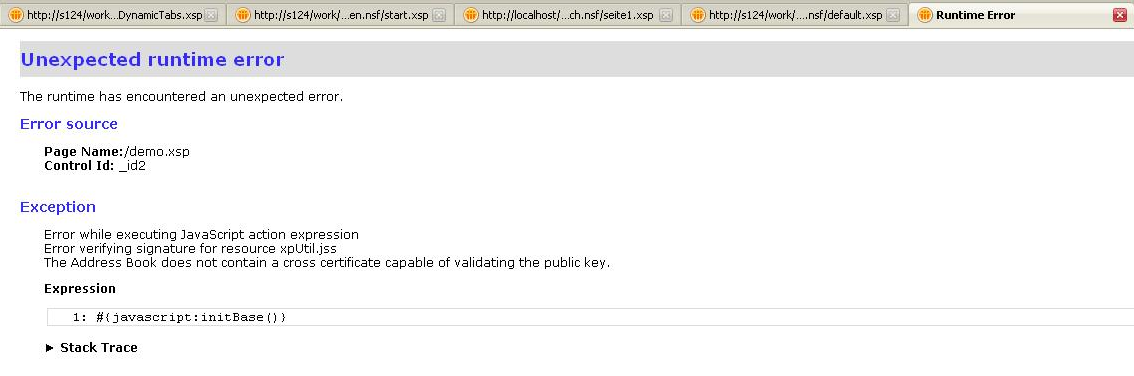
\includegraphics[scale=0.4]{pics/runtimeError}}
    \caption[Fehlermeldung - Unexpected runtime error]{\label{FiG:Unexpected-Runtime-Error }
	Im Browser angezeigte Fehlermeldung, Signatur Konflikt }
\end{figure} 

In Abbildung 6.1 ist eine Fehlermeldung ersichtlich. Dieser Fehler erscheint wenn, die Signaturen der Datenbank nicht übereinstimmen. Die Signatur des
Erstellers und des Benutzers sind nicht dieselbe. Mit dem Ergebnis, dass der Server die Datenbank nicht im Browser darstellen kann. 
\newline
\newline
Um diesen Konflikt zu vermeiden, sollten folgende Schritte eingehalten werden:
\begin{itemize}
\item Sollten im Designer bereits Design-Elemente geöffnet sein, müssen diese geschlossen werden.
\item Ändern der Signatur im Domino Administrator-Client 
\begin{itemize}
\item im Administrator das Verzeichnis der zu ändernden Datenbank auswählen
\item unter sign, den aktiven Benutzer(active user) \textbf{und} für alle Design-Elemente auswählen
\item sichern
\end{itemize}
\end{itemize}
\vspace{0.3cm}
Es besteht auch die Möglichkeit, jedes Designelement einzeln zu \textit{signen}, von dieser Möglichkeit ist jedoch abzuraten. 

%\footnote{Der Domino Administrator-Client ist für die Verwaltung von Domino Servern entwickelt
%worden. Dieser Client bietet Funktionen, welche mit dem Notes-Client nicht möglich sind.}